\documentclass[12pt]{article}

\usepackage{notestyle}

\graphicspath{{./img/}}


\title{Appunti Reti2}
\author{Brendon Mendicino}



\begin{document}

\maketitle
\newpage
\tableofcontents
\newpage


\section{Introduzione}\label{sec:introduzione}
...


\section{Multicast}
Gli indirizzi che identificano dei gruppi multicast sono quelli di tipo D, iniziano con 1110 ($224.0.0.0 - 239.255.255.255$).

Si prendono i 23 bit bassi dell'IP e vengono assegnati ai 23 bit bassi dell'indirizzo MAC multicast, questa operazione si chiama di \textbf{join} ad un gruppo multicast. Questo approccio potrebbe portare a dei conflitti, la probalit\`a che una collisione avvenga \`e molto bassa ma non \`e zero, i conflitti comportano ricevere il traffico di un altro gruppo multicast anche se non abbiamo fatto un join con quello.

Esempio: viene usato l'indirizzo 224.0.0.0 come un gruppo multicast, gli host che vogliono connettersi a questo gruppo dovranno fare il join, e quindi impostare la loro scheda di rete (solitamente una scheda di rete virtuale, in cui viene aggiunto il MAC multicast) con il MAC multicast, in questo caso gli ultimi 23 bit saranno a 0.


\section{IPv6}
Gli indirizzi ipv6 sono rappresentati su 128, quindi si hanno $2^{128}$ combinazioni. Per rappresentarli si divide l'indirizzo in 8 gruppi di 2 byte, separati da un ":". Ci sono delle strategie per rendere pi\`u leggibile l'indirizzo:
\begin{enumerate}
    \item gli zeri in fronte possono essere omessi;
    \item gli zeri (":0:") posso essere sostituiti con un "::" solo una volta;
\end{enumerate}

Per rappresentare l'indirizzo di rete si usano 64 bit. Il concetto di aggregazione gerarchico viene mentenuto del prefix length e dalla netmask, dunque il prefix viene usato per il subnetting.

I principi di assegnamento sono:
\begin{itemize}
    \item \textbf{subnetwork}: set of host with the same prefix;
    \item \textbf{link}: physical network;
    \item \textbf{on-link}: comunicazioni tra host con lo stesso prefisso;
    \item \textbf{off-link}: comunicazioni tra host con prefisso diverso;
\end{itemize}

\paragraph{Indirizzi Multicast}
Il multicast ha una rappresentazione simile ad IPv4, infatti hanno un range di FF00::/8, che si dividono in tre sottocategorie:
\begin{itemize}
    \item \textbf{well-known multicast}: FF00::/12, questo range di indirizzi \`e assegnato e quindi venduto, utilizzato per scopi di comunicazione;
    \item \textbf{transient}: FF10::/12, assegnati dinamicamente;
    \item \textbf{solicited-node multicast}: FF02:0:0:0:0:1:FF00::/104, simile al broadcast;
\end{itemize}
Un indirizzo multicast \`e formato da:
\begin{itemize}
    \tolerance=1000
    \item I primi 8 bit mi identificano un indirizzo multicast, tutti settati ad 1;
    \item 4 bit assegnati a dei flag: l'unico utilizzabile \`e il campo T che specifica se l'indirizzo \`e permanente (0), ovvero assegnato dalla IANA, oppure non-permanente (1), gli altri campi non hanno un'assegnazione;
    \item gli ultimi 112 rappresentano il \textbf{group id};    
\end{itemize}


4 bit per stabilire lo \textbf{scope} per difinire il range di indirizzi multicast;

\paragraph{Unicast}
Sono l'equivalte degli indirizzi publici IPv4. Quando un nuovo host si collega alla rete, sa automaticamente il suo indirizzo, infatti \`e gli indirizzi unicast sono plug and play. Gli indirizzi sono composti da:
\begin{itemize}
    \item 3 bit: 001;
    \item n bit: global routing prefix;
    \item m bit: subnet ID;
    \item 1280-m-n-3 bit: interface ID;
\end{itemize}

Il prefisso moderno \`e stato assegnato formalmente da entit\`a multi-livello:
\begin{itemize}
    \item 3 bit: 001;
    \item 13 bit: TLA ID, Top Level Authority (Large ISP);
    \item 32 bit: NLA ID, Next Level Authority (Organizzazione);
    \item 16 bit: SLA ID, Subnet Level Authority;
    \item 64 bit: Interface ID;
\end{itemize}


\paragraph{Link Local/Site Local}
Gli indirizzi link/site local sono assegnati automaticamente, iniziano con 1111 1110 1... (febf::/), allora:
\begin{itemize}
    \item link local: usati per gli indirizzi di rete per comunicare,
    \item site local: fec0::/10, indirizzi deprecati, utilizzati per assegnare degli indirizzi privati univoci;
\end{itemize}


\paragraph{Unique Local Address}
Gli ULA sono univoci, rimanendo comunque privati, e quindi non dovrebbero essre esposti alla rete, usando un range \`e di fc00::/7. La particolarit\`a \`e che l'ottavo bit \`e il \textbf{local flag} (L), se questo bit \`e settato ad 1 l'indirizzo \`e assegnato localmente, se invece \`e a 0 potrebbe essere assegnato in futuro. I successivi 40 bit sono asseganti casualmente, per mantenere l'univocit\`a.

\paragraph{IPv4 Embedded Address}
Sono usati per rappresentare gli indirizzi ipv4 sugli indirizzi ipv6. Sono composti da:
\begin{itemize}
    \item i primi 80 bit a 0;
    \item 16 bit a 1;
    \item gli ultimi 32 bit rappreesntano l'indirizzo ipv4;
\end{itemize}

\paragraph{Loopback Address}
L'indirizzo ::1 ha lo stesso scopo dell'indirizzo di loopback 127.0.0.1 di ipv4.

\paragraph{Unspecified Address}
\`E un indirizzo unicast non specificato ::0, anche in questo caso il suo comportamento \`e lo stesso di ipov4.


\paragraph{Indirizzi Anycast}
Ho degli indirizzi assegnati a dei nodi nelle rete e quando mando un pacche voglio che esso arrivi ad uno di essi (inizialmento pensato per i DNS server). Gli indirizzi anycast non sono utilizzati.


\newpage
\subsection{Protocolli IPv6}
In ipv6 alcuni protocolli sono stati integrati o rimossi rispetto ad ipv4, infatti ARP ed IGMP sono stati integrati in ICMP, la maggior parte degli altri protoccolli \`e stata fatta una modifica per supportare gli indirizzi a 128 ma le modifiche rimangono minime.

\subsubsection{IP}
L'header in ipv6 contiene molte meno dati, il motivo \`e che le informazioni sono presenti nel padding, tutto ci\`o \`e possibile grazie al campo next header. Si crea cos\`i una catena di header. Se non ho bisogno di estensioni allora il campo next header punter\`a all'header tcp.
\begin{figure}[H]
    \centering
    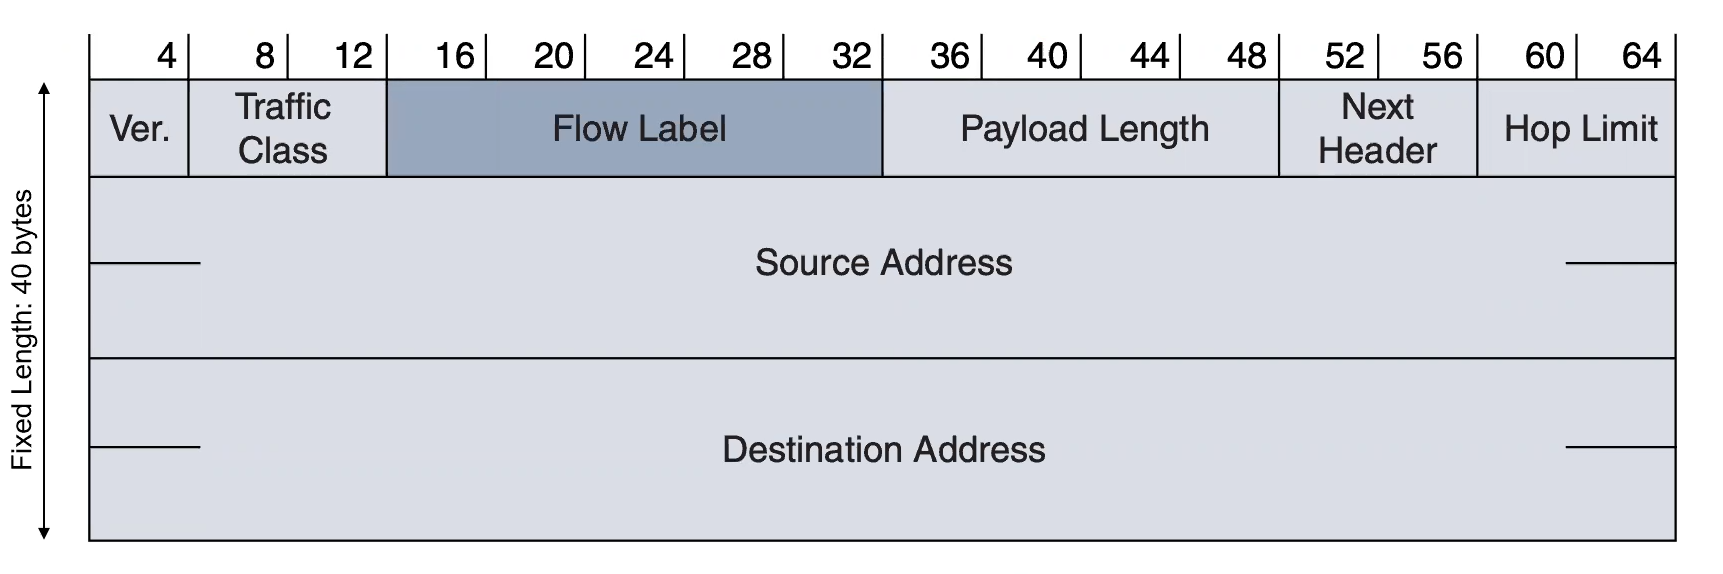
\includegraphics[width=0.8\textwidth]{ipv6-header.png}
    \caption{Ipv6 Header}
    \label{fig:ipv6-header}
\end{figure}
I campi rimasti sono:
\begin{itemize}
    \item ver: la versione del protocollo;
    \item traffic class: si definiscono delle classi di pacchetti per determinare delle priorit\`a tra i traffici;
    \item flow label: etichetta associata al flusso, sar\`a possibile fare routing grazie a questo campo;
    \item payload lenght: lunghezza del payload;
    \item hop limit: time to live del ipv4;
    \item source address;
    \item destinatoin address;
\end{itemize}

\paragraph{Headers extensions}
Il protocollo utilizza dei codici per specificare quale sar\`a il campo dell prossima estensione.
\begin{figure}[H]
    \centering
    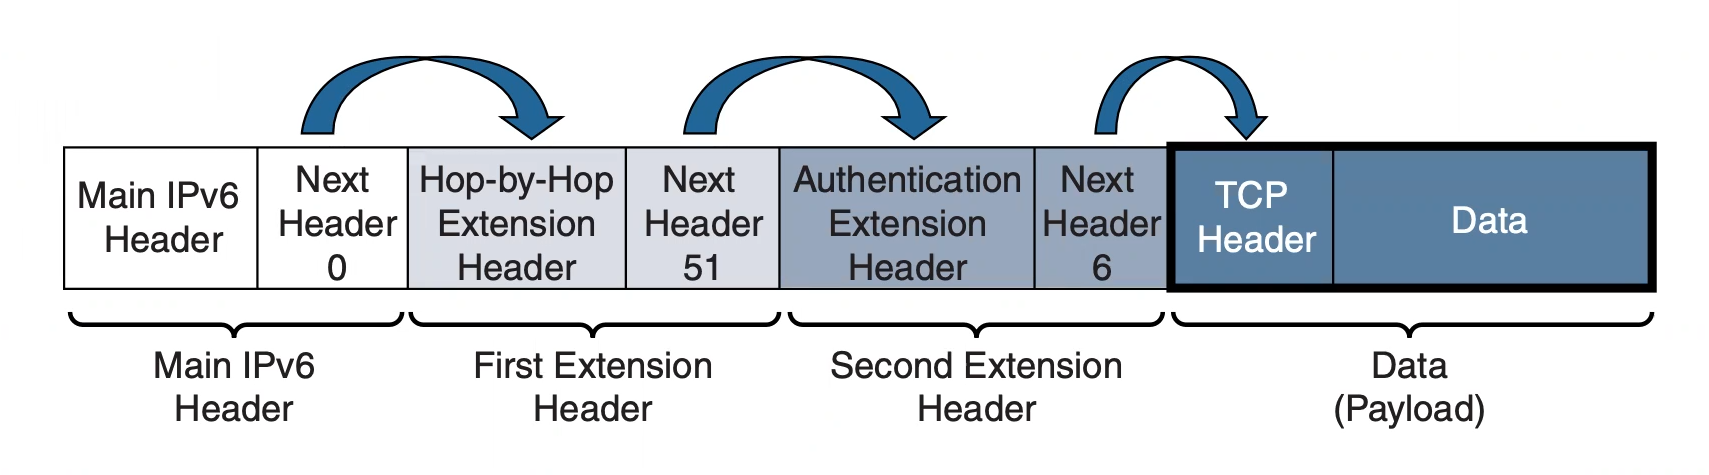
\includegraphics[width=0.8\textwidth]{header-chaining.png}
    \caption{Header Chaining}
    \label{fig:header-chaining}
\end{figure}
Gli header hanno tutti lo stesso formato:
\begin{itemize}
    \item next header;
    \item length: pi\`u o meno dato dell'header;
    \item extension data: dati dell'header;
\end{itemize}


\subsubsection{Interfaccia con i livelli pi\`u bassi}
Nel livello si \`e deciso di differenziare il protocllo ipv4 e ipv6 (approccio dual stack), infatti nel livello 2 esiste un campo che specifica il protocollo a livello superiore. Il \textbf{type} per ipv6 \`e 86DD.

\subsubsection{Mapping}
\tolerance=1000
I 32 bit bassi dell'indirizzo ipv6 vengono mappati ai 32 bit bassi dell'indirizzo MAC, questo mapping viene specificato quando i primi 2 byte sono settati a 33:33, dunque un indirizzo MAC mappato sar\`a 33:33:xx:xx:xx:xx. Quanso si manda un pacchetto all'indirizzo di broadcast ff0c::89:aabb:ccdd l'indirizzo MAC corrispondente sar\`a 33:33:aa:bb:cc:dd.

\subsubsection{Neigbhor Discovery}
Il protocollo ARP sar\`a sostituito dalla nuova version del protocollo ICMPv6.

Il meccanismo avviene nel seguente modo: partendo da un indirizzo unicast si prendono i 24 bit bassi dell'indirizzo e si crea un indirizzo multicast solicited-node con i 24 bit bassi corrispondenti a quelli dell'unicast. Questo permette, quando si fa il mapping, di avere gli indirizzi MAC multicast che iniziano con 33:33:ff, grazie a come sono composti gli indirizzi solicited-node.
\begin{figure}[H]
    \centering
    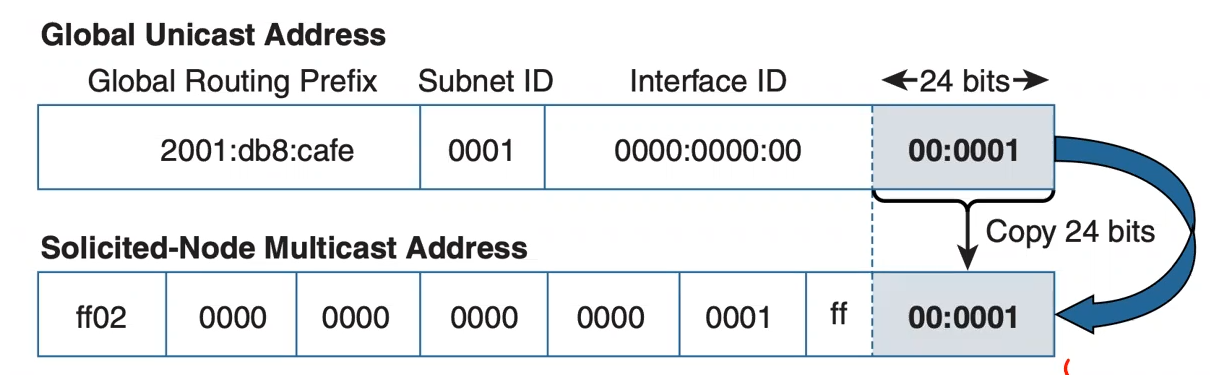
\includegraphics[width=0.8\textwidth]{solicited-node-multicast-address.png}
    \caption{Solicited Node Multicast Address}
    \label{fig:solicited-node-multicast-address}
\end{figure}

ARP:
\begin{itemize}
    \item manda un trama in broadcast;
\end{itemize}

Multicast:
\begin{itemize}
    \item manda a tutti;
    \item manda solo a chi fa parte di un gruppo: il MAC di multicast permette di mandare messaggi solo a chi appartiene a chi potenzialmente fa parte di quel gruppo;
\end{itemize}


\subsection{ICMPv6}
Il protocollo mantiene le opzioni di quello usato in ipv4 aggiungnendo delle funzionalit\`a per sostituire ARP e IGMP, ICMP \`e usato per:
\begin{itemize}
    \item diagnostica;
    \item neighbor discovery;
    \item multicast group;
    \item issue notification;
\end{itemize}

\subsubsection{Formato del messagio}
ICMP \`e incapsulto nel pacchetto ip.
\begin{figure}[H]
    \centering
    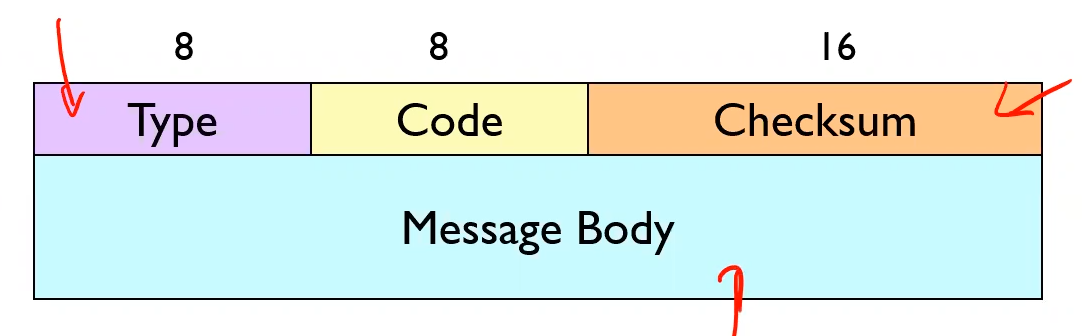
\includegraphics[width=0.8\textwidth]{icmp-format.png}
    \caption{Icmp Format}
    \label{fig:icmp-format}
\end{figure}
Messaggi di errore:
\begin{itemize}
    \item 1: destination unreachable;
    \item 2: packet too big;
    \item 3: time exeeded;
    \item 4: parameter problem;
\end{itemize}
Echo:
\begin{itemize}
    \item 128: echo request;
    \item 129 echo: reply;
\end{itemize}

\paragraph{Neighbor Solicitation}



\paragraph{Neighbor Advertisement}
Vengono aggiunti 3 flag:
\begin{itemize}
    \item router: indica se il pacchetto arrivo da un router;
    \item solicited: specifica se il nodo \`e stato sollicitato o meno;
    \item override: specifice se l'host cache deve essere sovrascritta;
\end{itemize}
L'indirizzo MAC viene messo nel campo options, mente l'ip di sorgente viene messo nel campo target address.

\subsubsection{Group Management}
Da rivedere...
\begin{itemize}
    \item query;
    \item report;
    \item done;
\end{itemize}

\subsection{Configurazione}
Le informazioni necessarie sono:
\begin{itemize}
    \item address prefix;
    \item interface id;
    \item default gateway;
    \item dns server;
    \item host name;
    \item domain name;
    \item MTU maximux transmission unit;
\end{itemize}
Per creare queste informazioni:
\begin{itemize}
    \item stateful config: informazioni date da un DHCP;
    \item stateless config: generate automaticamente;
    \item ibrida (stateless DHCP);
\end{itemize}

\subsubsection{Interface ID}
Si pu\`o configurare manualmente, ottenere dal DHCP oppure generati automaticamente. Nel modo di configurare i 64 bit bassi non si hanno garanzie che siano univoci, esiste un protocollo che permette il controllo e l'univocit\`a.

\paragraph{EUI-48 to EUI-64 Mapping}
EUI = Extended Unique Id

OUI = Organization Unique Id

Per creare l'interface ID in modo automatico si pu\`o sfruttare la tecnica del mapping, si prende il MAC del interfaccia e viene mappato nel seguente modo:
\begin{figure}[H]
    \centering
    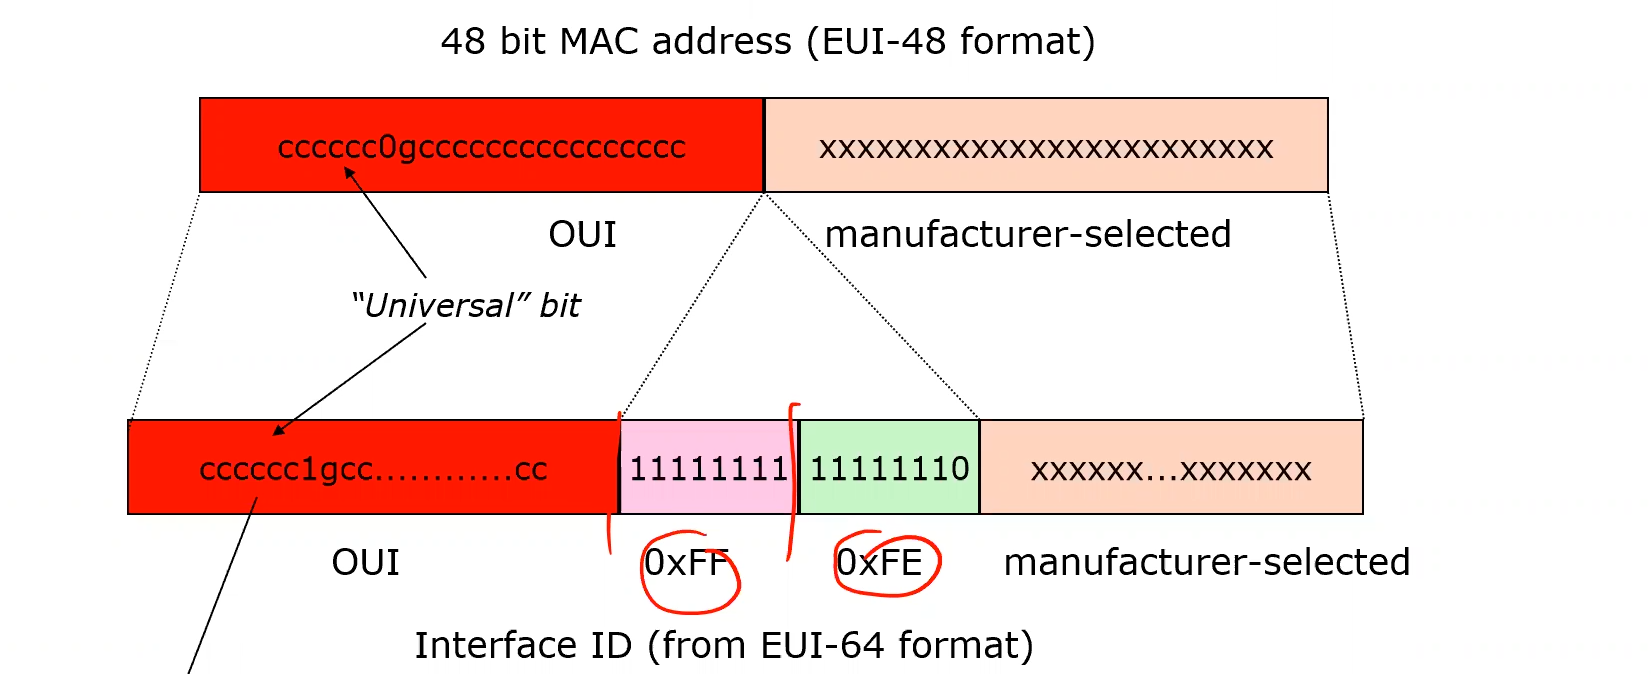
\includegraphics[width=0.8\textwidth]{mac-to-id-mapping.png}
    \caption{Mac To Id Mapping}
    \label{fig:mac-to-id-mapping}
\end{figure}
Il settimo bit viene settato a 0 se l'ID viene assegnato automaticamente, mentre viene settato a 1 se l'ID \`e stato assegnato manualmente (quidni l'indirizzo sar\`a necessariamente univoco), questa \`e una convenzione ma non la regola.

\paragraph{Privacy Extension Algorithm}
Per evitare che l'interface Id possa essere calcolato da qualcun'altro ch conosca il MAC del mio dispositivo si usa un approccio per garantire maggior privacy ed aumentare la sicurezza.

Per generare l'interface Id si prendono 64 bit random e 64 bit generati del MAC mapping e poi viene fatto un hash. In fine il settimo bit viene settato a 0 perch\'e non si ha comunque la certezza che l'interface Id sia univoco.
\begin{figure}[H]
    \centering
    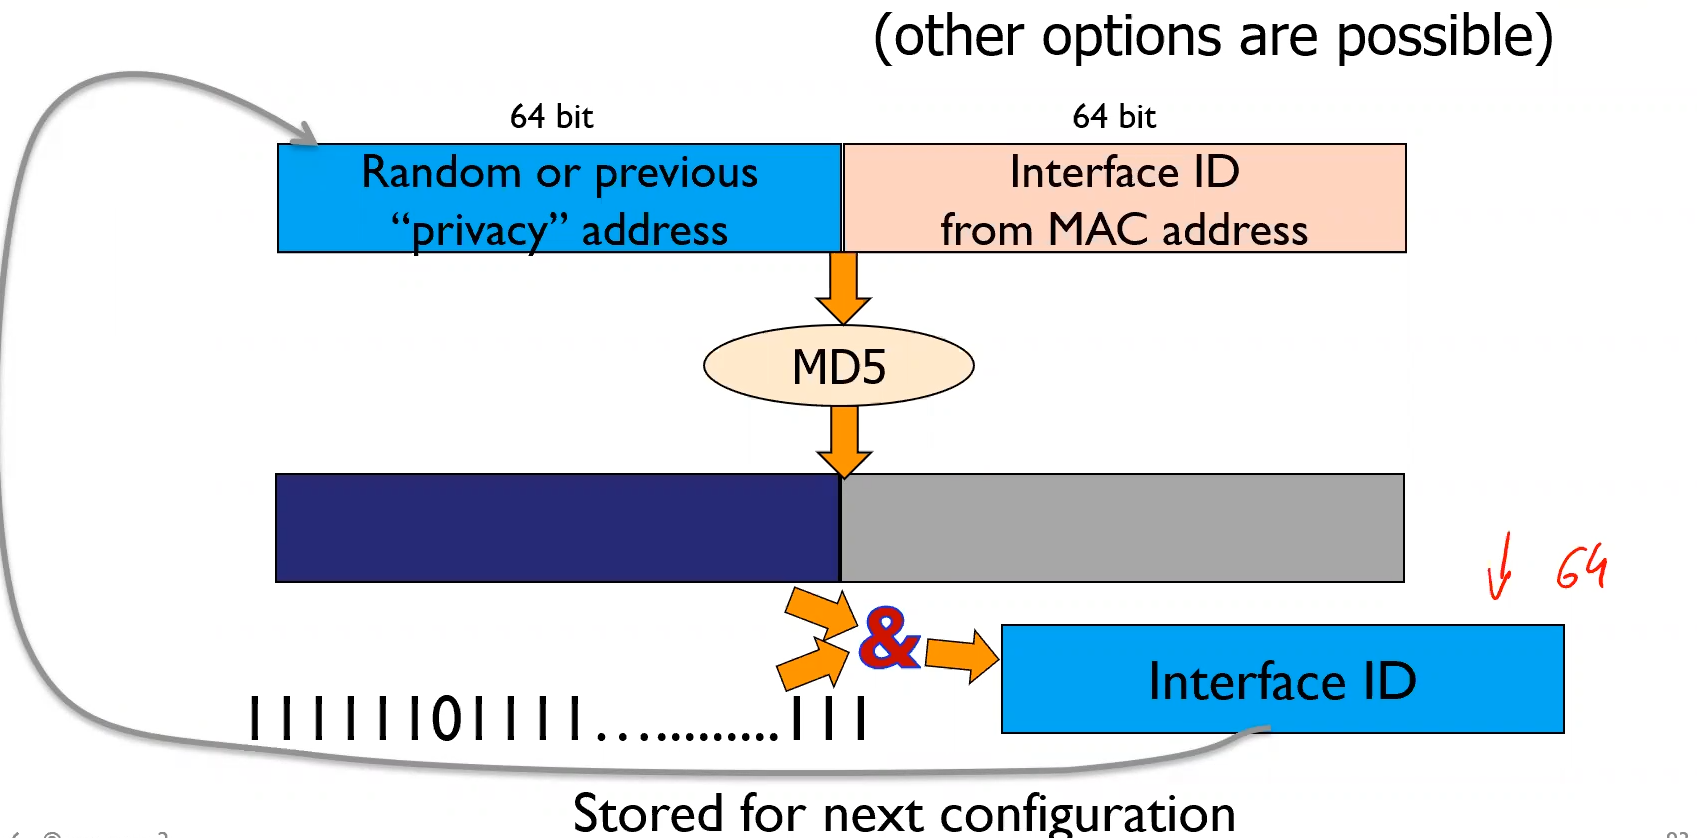
\includegraphics[width=0.8\textwidth]{privacy-extension-alogorithm.png}
    \caption{Privacy Extension Alogorithm}
    \label{fig:privacy-extension-alogorithm}
\end{figure}


\subsubsection{Address Prefix}
Anche in qeusto caso \`e possibile configurare la parte alta dell'indirizzo ip in modo manuale oppure in modo automatico.

Per ottenere queste informazioni in modo automatico esistono due messaggi:
\begin{itemize}
    \item \textbf{Router Solicitation}: nelle opzioni solitamente si chiede l'indirizzo
        \begin{figure}[H]
            \centering
            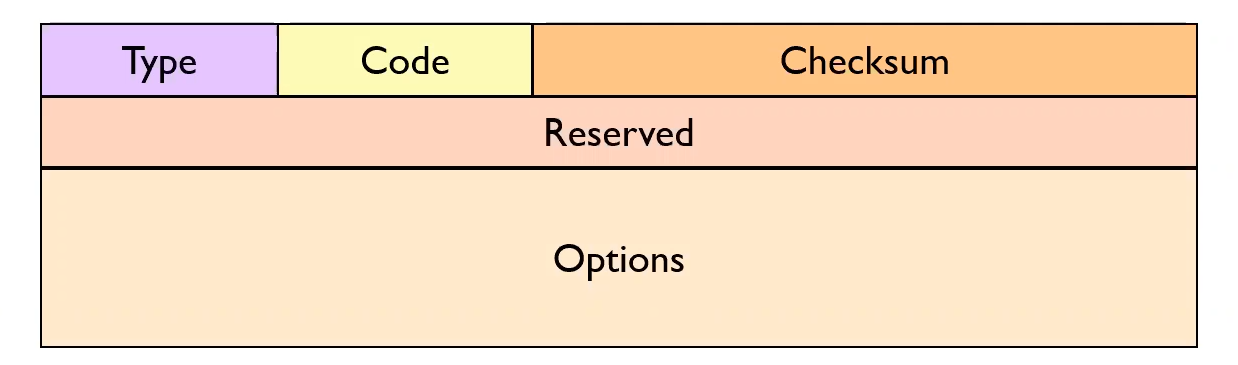
\includegraphics[width=0.8\textwidth]{router-solicitation.png}
            \caption{Router Solicitation}
            \label{fig:router-solicitation}
        \end{figure}
    \item \textbf{Router Advertisement}: pu\`o essere una risposa ad una solicitaion, M (Managed Address Configuration): se settato ad 1 indica che l'indirizzo \`e disponibile via DHCP; O (Other Configuration): parametri come il DNS server; Reachable Time: tempo in cui il router \`e disponibile; Retrans Timer: tempo in cui l'indirizzo \`e disponibile;
        \begin{figure}[H]
            \centering
            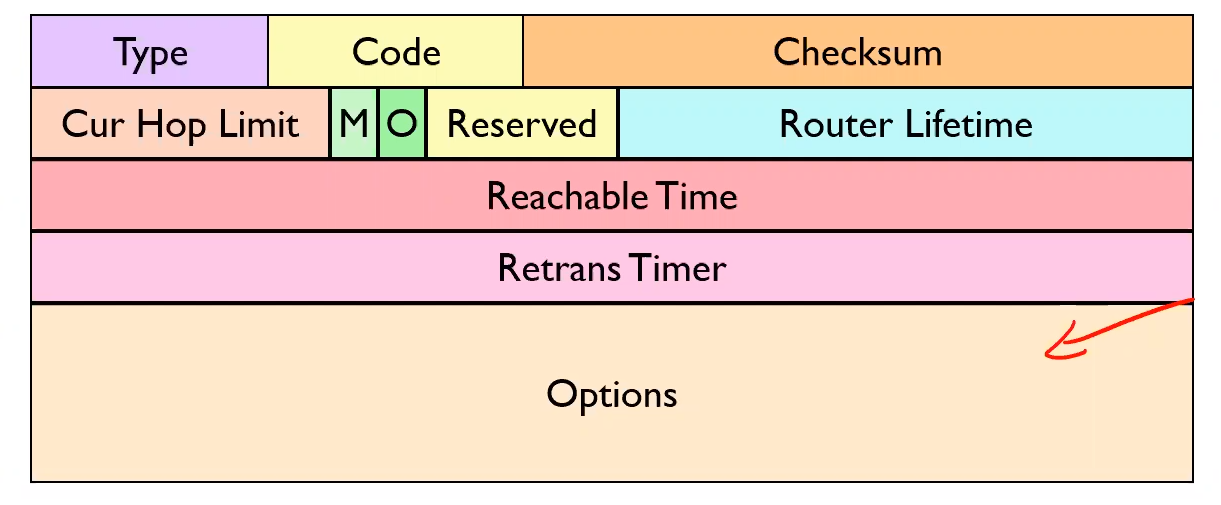
\includegraphics[width=0.8\textwidth]{router-advertisement.png}
            \caption{Router Advertisement}
            \label{fig:router-advertisement}
        \end{figure}
\end{itemize}
Quando un host si collega ad una rete potr\`a fare una solicitation e ricevere una advertisement oppure i router periodicamente mandano una advertisement.

Le informazioni sul prefisso sono:
\begin{itemize}
    \item L: ad 1 se il prefisso pu\`o essere on-link;
    \item A: ad 1 se il prefisso pu\`o essere usato con una configurazione autonoma;
\end{itemize}

Un'altra informazione \`e il \textbf{Link Layer Address Option}, si mette il MAC del default gateway.

Un messaggio molto importante \`e l'\textbf{ICMP Redirect}, in una rete ci sono pi\`u router, l'host manda i pacchetti al suo default gateway, se per raggiungere un altro host un altro \`e router \`e pi\`u vicinino allora i pacchetti vengono rediretti in quel router.

\subsubsection{Duplicate Address Detection (DAD)}
L'host manda un messaggio di DAD. 
Per verificare che non esistano indirizzi duplicati ...


\subsection{Stateless Config}
Il link local address viene generato automaticamente, successivamente viene fatta una DAD, l'host si iscrive al Solicited Node Multicast Address, abilita le comunicazioni on-link.

Una volta acquisita la parte bassa si ottiene la parte alta: router solicitation, router advertisement listening, si crea il prefisso dall'adversement, si fa una DAD, ci si iscrive al Soliced Node Mutlicast Address.

Un altra grosso vantaggio \`e il \textbf{Renumbering}, tramite l'advertisement si riassegnano gli indirizzi in modo automatico.

\subsection{Stateful Config}
La configurazione stateful rimane invariata tranne che per le informazioni date dal flag M.
...


\section{Scope}
Qunado un dispositivo ha pi\`u interfaccie, gli indirizzi generati automaticamente saranno gli stessi, per distinguere le due interfacce l'host tiene conto a quale interfaccia mandare un messaggio. Per distinguere le due interfaccie si mette \%x, dove x \`e l'id dell'interfaccia.



\section{IPv6 Transitioning}
\subsection{IPv4 Traversing}
Si fa del \textbf{Tunneling}, partendo da un paccheto ipv6 che si interfaccia ad una rete ipv4, si parte da un indirizzo ipv4 e nul suo header viene encapsulato l'indirizzo ipv6. Le soluzioni ci permettono di avere un mapping automatico o manule:
\begin{itemize}
    \item \textbf{IPv4-compatible}: quando devo inviare un messaggio a destinazione gli ultimi 32 bit dell'indirizzo ipv6 sono i bit dell'indirizzo ipv4 (::/96);
    \item \textbf{6over4}: sfrutta il multicast dell'ipv4 e dell'ipv6;
    \item \textbf{ISATAP}: si basa su un prefisso comune (fe80::5efe) e gli ultimi 32 bit come l'indirizzo ipv6,
    \item ...
\end{itemize}




\section{Wireless and Cellular Networks}
\subsection{Wireless LAN}
Le caratterisiche del link wireless sono:
\begin{itemize}
    \item un link Wireless ha un degrado maggiore del segnale, rispetta ad una fibra ottica;
    \item \`e soggetto a interferenze;
    \item problema del \textbf{fading}, causato dai rimbalzi del segnale su ostacoli;
\end{itemize}
Esistono vari standard dello IEEE 802.11 wireless LAN, i pi\`u moderni arrivano fino a 5GHz, il problema con le alte frequenze \`e 

Tutte le implementazioni utilizzano il protocollo di accesso \textbf{CSMA/CA}.

Un \textbf{access point} o una \textbf{base station} serve una \textbf{Basic Service Set (BSS)}, dentro la BSS si trovano sia gli access point che gli host.
\begin{figure}[H]
    \centering
    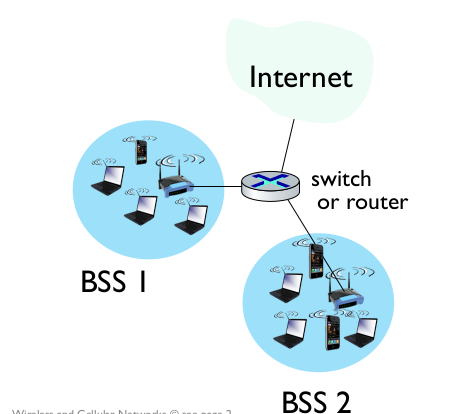
\includegraphics[width=0.8\textwidth]{bss.png}
    \caption{BSS}
    \label{fig:bss}
\end{figure}

Un dispositivo fa il \textbf{sensing} per cercare un canale operativo, che provengono di vari access point, ascoltando per il \textbf{beacon frame} che serve ad agganciarsi ad un access point, ci sono diversi beacon fram ed il dispositivo si collega all'access point con il segnale pi\`u forte, il beacon frame contiene:
\begin{itemize}
    \item il nome dell'AP (SSID);
    \item l'indirizzo MAC;
\end{itemize}
Per poter accedere ad una rete wifi, oggigiorno, hanno tutte bisogno di autenticazione, e tipicamente sar\`a presente un DHCP per ottenere una configurazione IP.

\subsection{CSMA/CA}
Il protocollo fa il sensing del canale (CSMA = carrier sense multiple access), ed la collision avoidance (CA), il motivo \`e che in una rete wireless il mezzo di trasmissione \`e l'aria che \`e un mezzo condiviso. 
Il sender:
\begin{itemize}
    \item si fa il sense del canale, si aspetta un tempo di DIFS e si trasmettono i dati;
    \item se si fa il sense ed il canale \`e occupato si aspetta, per applicare la CA parte un randon exponential backoff timer quando sento il canele occupato (in ethernet il timer partiva solo quando avveniva una collisione!);
\end{itemize}

Per evitare le collisione gli hots mandano un piccolo pacchetto , per sprecare la minor banda possibile, detti RTS (ready to send) usando CSMA, l'AP rispondono in broadcast agli host con un CTS (clear to send) per un degli host che ha mandato l'RTS, dopich\`e l'host a cui l'AP ha mandato il CTS che inizia a trasmettere una trama e l'AP manda sempre in broadcast un ACK all'host che ha trasmesso la trama.
\begin{figure}[H]
    \centering
    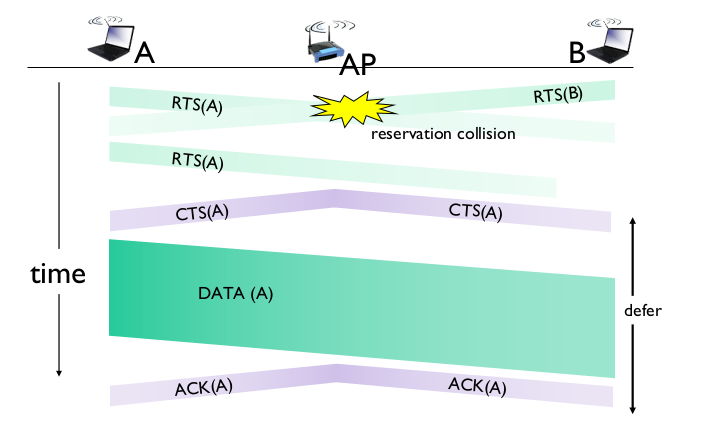
\includegraphics[width=0.8\textwidth]{collision-avoidance.png}
    \caption{Collision Avoidance}
    \label{fig:collision-avoidance}
\end{figure}

Una trama 802.11 \`e fatta da:
\begin{itemize}
    \item frame control: \`e composto da:
        \begin{itemize}
            \item protocal version;
            \item type: RTS, CTS, ACK, data;
            \item power mgt;
            \item ...;
        \end{itemize}
    \item duration: la durata che ci mette la trama per essere trasfertita;
    \item address 1: indirizzo dell'interfaccia MAC dell'AP, il motivo per cui \`e presente questo indirizzo \`e che nelle reti wireless bisogna prima passare dell'AP (violando in qualche modo il principio su cui si basa il livello link nelle reti ethernet, dove se uno swith \`e presente il pacchetto viene direttamente inoltrato al mac di destinazione, senza passare dal router);
    \item address 2: indirizzo sorgente;
    \item address 3: indirizzo dell'interfaccia del router a cui l'AP \`e collegato;
\end{itemize}
\begin{figure}[H]
    \centering
    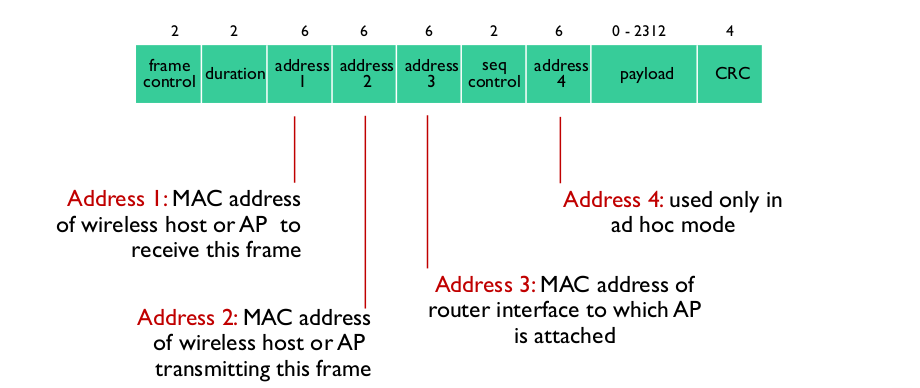
\includegraphics[width=0.8\textwidth]{802.11-frame.png}
    \caption{802.11 Frame}
    \label{fig:802.11-frame}
\end{figure}

In una rete wireless va gestita anche la mobilit\`a, questo \`e improbabile in una rete wifi, solitamente il movimento \`e fatto in una subnet, ovvero in una rete in cui sono presenti pi\`u AP collegati allo stesso router di una sottorete.

Un'altra capacit\`a dei dispositivi \`e il poter entrare in \textbf{sleep mode}, un nodo manda all'AP questa richiesta, se l'AP riceve delle trame da mandare al nodo li bufferizza finch\'e il nodo non si svelgia, un nodo si riattiva quando un beacon frame viene mandato, nel beacon frame vengono anche segnalati gli host per cui ci sono dei messagi in coda, allora il nodo capisce che deve svegliarsi e colleziona le trame, oppure continua a dormire.


\subsection{Cellular Networks}
Una rete cellulare \`e una rete che cerca di coprire un'area geografica molto vasta attraverso le \textbf{celle}, dove il terminale utente si muove anche su lunghe distanze, gestendo il cambiamento du una cella all'altra, detto \textbf{handover}.

La forma e le dimsioni di una cella sono determinate da:
\begin{itemize}
    \item potenza emessa;
    \item altezza;
    \item il guadagno dell'antenna: indica quanto un'antenna \`e buona nella trasmissione;
    \item morfologia del territorio;
    \item condizioni di propagazione: se nevica il segnale sar\`a pi\`u attenuato;
\end{itemize}
Le celle utilizzate in pratica sono:
\begin{itemize}
    \item Una \textbf{macrocella} viene relizzata con un'antenna posizionata molto in alto;
    \begin{figure}[H]
        \centering
        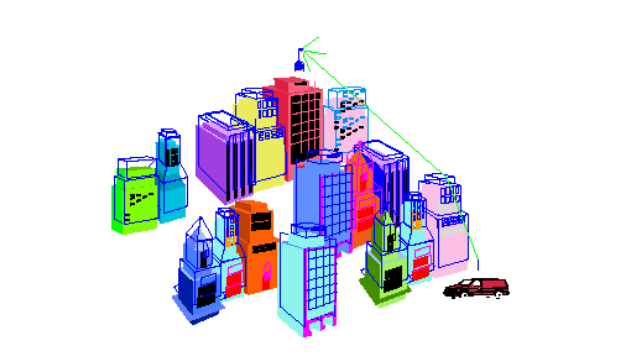
\includegraphics[width=0.6\textwidth]{macrocella.png}
        \caption{Macrocella}
        \label{fig:macrocella}
    \end{figure}
    \item \textbf{Microcella} realizzata con antenne non molto posta in alto,
    \begin{figure}[H]
        \centering
        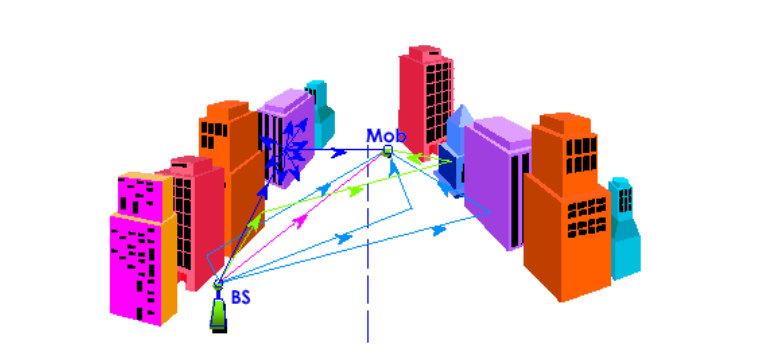
\includegraphics[width=0.6\textwidth]{microcella.png}
        \caption{Microcella}
        \label{fig:microcella}
    \end{figure}
\end{itemize}

Nelle reti cellulari non si usa CSMA/CD, le tecniche di condivisione sono: fdma, tdma, cdma, sdma. Per quasi tutte le reti cellulari si usa FDMA con riutilizzo dell frequenze, sfruttando la distanza fisica che separe le celle. Vengono creati dei \textbf{cluster} di celle in cui vengono usate tutte le frequenze disponibili, al di fuori di questo cluster si possono riutilizzare le frequenze, il numero di celle presenti in un cluster si indica con G=x. Nei cluster le celle che hanno le stesse frequenze si chimano \textbf{co-channel}.
\begin{figure}[H]
    \centering
    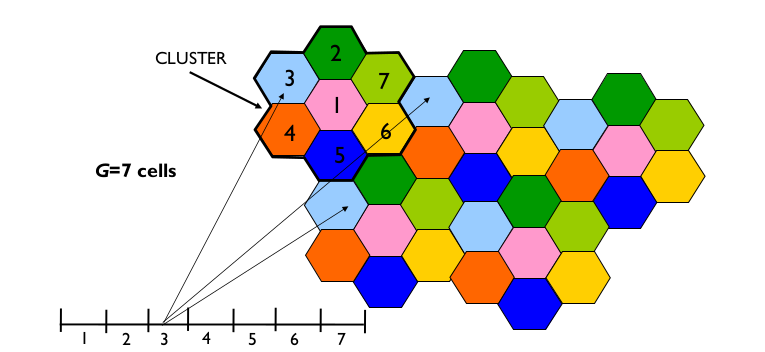
\includegraphics[width=0.8\textwidth]{7-cell-cluster.png}
    \caption{7 Cell Cluster (G=7)}
    \label{fig:7-cell-cluster}
\end{figure}
Per soddisfare pi\`u utenti si possono diminuire le dimensioni delle celle, soddisfando meno utenti per area ma incrementando l'ottimizzazoine di utilizzo delle frequenze, se per\`o si inzia a diminuire troppo la dimensione sorgono dei problemi:
\begin{itemize}
    \item aumento dei costi per creare le maggiori celle;
    \item diminuendo il numero di celle in un cluster aumento l'interferenza, la distanza tra i co-channel diventa pi\`u piccola, creando interferenze maggiori nella stessa frequenza;
\end{itemize}

Tecniche di freqency reuse:
\begin{itemize}
    \item \textbf{Splitting}: coesistenza di microcelle e macrocelle, esempio: in campagna sarebbe meglio gestita con macrocelle pi\`u copertura e meno persone da gestire, in citt\`a ha pi\`u senso usare delle micro celle, meno copurtura per pi\`u utenti da gestire e pi\`u ostacoli da evitare;
    \item \textbf{Cell Shaping}: per evitare degli handover mette le micro celle in posti dove le persone so che rimarranno ferme, e per le persone che si muvono avr\`o delle macrocelle che caoprono un area pi\`u ampia;
    \item \textbf{Power Control}: \`e una tecnica per evitare di sprecare pi\`u batteria del necessario, per decidere la potenza da utilizzare; le strategia sono: open loop, closed loop, ...; nell'open loop 
    \item \textbf{Sectoring}: si vanno a considerare delle antenne con capacit\`a di trasmissioni non omnidirezionali, diminuendo le interferenze in una certa direzione;
    \item \textbf{Tilting}: non usare un angolo di 90 gradi per le trasmissioni, limitando le interferenze;
    \item \textbf{Creating femtocell}: si creano delle celle al volo quando ne ho bisogno dove ne ho bisogno, esempio: uno stadio non avrebbe senso di essere gestito ogni giorno della settimana, se non quando lo stadio si riempe di gente per un evento;
\end{itemize}

jArchittura ...

\subsection{Basi Procedures}
\begin{itemize}
    \item \textbf{Registrazione}: fornire un associazione ad un rete cellulare, la registrazione viene fatta ogni qual volta un utente voglia accedere ad un servizione;
    \item \textbf{Mobilit\`a}: le procedure legate alla mobilit\`a sono:
        \begin{itemize}
            \item \textbf{Roaming}: il roaming \`e la capacit\`a di un terminale di essere tracciabile in una rete, tenendo i log su ogni cella in cui \`e stato attaccato. Per effettuare il roaming la rete ricorda in quale location area il terminale si trova, pi\`u celle adiacenti formano una lacation area, non \`e detto che una location area sia fatta da celle di un solo opertatore. Ognuna di queste lacation area ha un ID detto Location Area Id (LAI);
            \item \textbf{Location updating}: \`e l'operazione che un utente deve fare ogni qual volta si muove e cambia location area, un treminale si accorge di aver cambiato LA quando visualizza un LAI diverso;
            \item \textbf{Paging}: come si fa ed essere tracciabili? La rete conosce la LA in cui il terminale si trova, ma non la specifica cella, allora quando arriva un messagio per host x, il sistema manda un \textbf{paging message} in broadcast in tutta la LA (simile ad un ARP request), il motivo per cui si manda un messaggio in broadcast in una location area \`e limitare il numero delle laction updating;
            \item \textbf{Handover}: procedura molto complessa per continuare a mantenere la connessione passando da una cella all'altra, si classificano in: intra-cella vs inter-cella, (soft vs hard) sono collegato ad entrambe le base station, sono collegato prima ad una e poi ad un altra, (MT vs BS) inizializzata da MT a dalla BS (tipicamente), (Backward vs Forward) procedure gestite dalla cella di arrivo o dalla cella di partenza;
        \end{itemize}
\end{itemize}








\end{document}
